% https://stuff.mit.edu/afs/athena/contrib/tex-contrib/beamer/pgf-1.01/doc/generic/pgf/version-for-tex4ht/en/pgfmanualse12.html
\documentclass[12pt,ngerman]{scrartcl}

\usepackage[]{babel}
\usepackage[]{tikz}
\usetikzlibrary{arrows}


\begin{document}

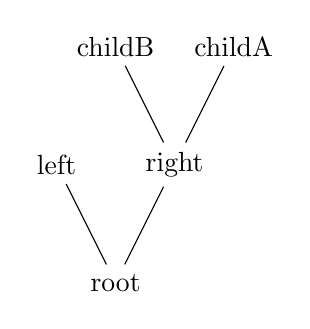
\begin{tikzpicture}
  \node {root}[grow'=up]
    		child {
    			node {left}
    		}
    		child {node {right}
      			child {
      				node {childB}
      				}
      			child {
      				node {childA}
      				}
    	};
\end{tikzpicture}


\begin{tikzpicture}[level distance=2cm]
  \tikzstyle{level 1}=[sibling distance=8cm]
  \tikzstyle{level 2}=[sibling distance=4cm]
  \tikzstyle{level 3}=[sibling distance=3cm]
  \coordinate
    child foreach \x in {0,1}
      {child foreach \y in {0,1}
        {child foreach \z in {0,1}}};
\end{tikzpicture}

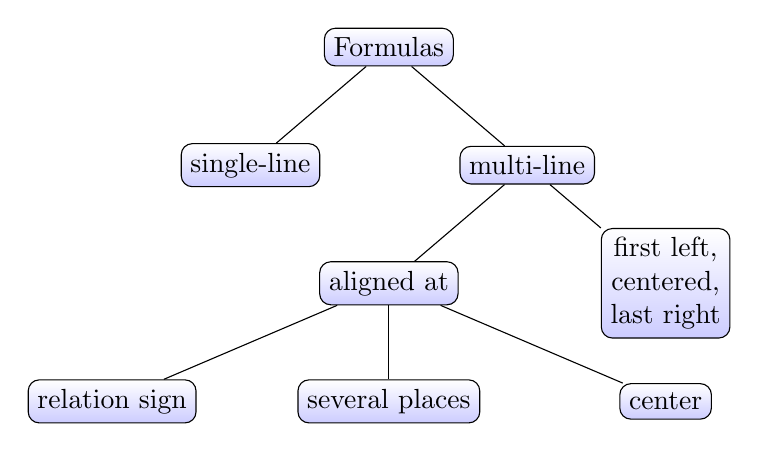
\begin{tikzpicture}[sibling distance=10em,
  every node/.style = {shape=rectangle, rounded corners,
    draw, align=center,
    top color=white, bottom color=blue!20}]]
  \node {Formulas}
    child { node {single-line} }
    child { node {multi-line}
      child { node {aligned at}
        child { node {relation sign} }
        child { node {several places} }
        child { node {center} } }
      child { node {first left,\\centered,\\last right} } };
\end{tikzpicture}

\end{document}